\section{Event Preselection and Reconstruction}
To suppress SM backgrounds while keeping the signal events at high efficiency, event selection criteria are made to select interesting events in the datasets. Preselection criteria are used to define a control region to help optimize the background modeling. Afterwards, further selections are made to define the signal region. These will be discussed in Section~\ref{sec:selection_sr}.

\subsection{Lepton Selection}
Electrons and muons are selected from both single lepton datasets and the MC simulation samples, and paired to be reconstructed as a Z boson candidate. The detailed selections in addition to the single lepton HLT requirements are described below.
\subsubsection{Electron Pair Selection}
Both electrons in a selected electron pair are required to pass the Egamma loose cut-based Identification and Isolation as described in Section~\ref{sec:ob_eidiso} to be regarded as a well-identified electron. Additional criteria are required on the $p_T$ and $\eta$ values of the leading and subleading electrons in the pair, as listed below.
\begin{enumerate}
\item Leading Electron: $p_T >120\GeV$, $|\eta|<2.5$
\item Subleading Electron: $p_T >35\GeV$, $|\eta|<2.5$
\end{enumerate}

The restriction on their $|\eta|$ value is due to the design of the ECAL detector. And for the leading electron, only those with $p_T$ beyond 120\GeV will be kept, because the single electron HLT (\texttt{HLT\_Ele115\_CaloIdVT\_GsfTrkIdT}) we use has a threshold at 115\GeV. More discussion can be found in Section~\ref{sec:bkg_trig}.

\subsubsection{Muon Pair Selection}\label{sec:muonselection}
Two muon identification approaches are involved in the muon pair selection to optimize the muon pair selection efficiency, as described in Section~\ref{sec:ob_midiso}. Various combinations of muon IDs are considered. Figure~\ref{fig:sel_mumueff} shows the muon pair efficiencies for different muon ID combinations versus $\Delta R$ between the two muons in the pair and the $p_T$ of the muon pair.

\begin{figure}[htbp]
\begin{center}
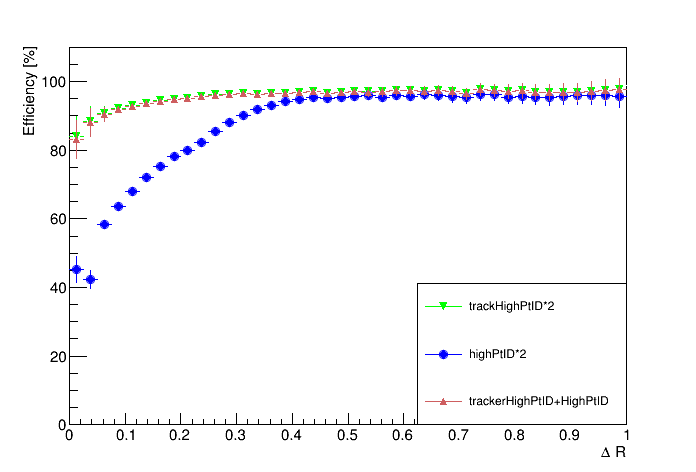
\includegraphics[width=0.9\linewidth]{figures/sel_mudreff.png}
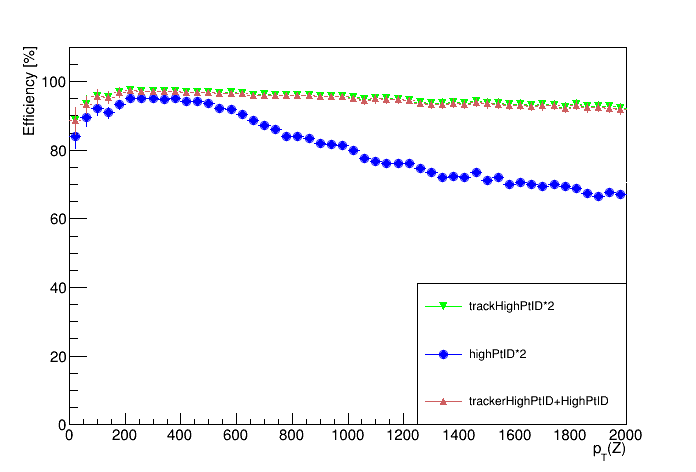
\includegraphics[width=0.9\linewidth]{figures/sel_muzpteff.png}
\caption{Efficiency comparison among various muon ID combinations, versus $\Delta R$ between the muons (upper) and $p_T$ of the muon pair (lower).}
\label{fig:sel_mumueff}
\end{center}
\end{figure}

\vspace{0.3cm}
The efficiency profiles are obtained from the signal MC samples generated by Madgraph, and generator level information is used to judge if a reconstructed muon is a true muon or not. The two efficiency plots are consistent considering the fact that the $\Delta R$ between the muons is likely to be smaller in a pair with higher $p_T$. From the plot one can see huge sacrifice in efficiency by requiring both muons to pass the High $p_T$ ID, because the resolution of the muon system is not high enough to distinguish the two adjacent muons and reconstruct them as separated tracks. However, the other two ID combinations (two Tracker High $p_T$ ID combination and Tracker High $p_T$ ID $+$ High $p_T$ ID combination) perform with much higher efficiency in the high $p_T$ region. Considering that the High $p_T$ ID is a tighter identification compared to the tracker High $p_T$ ID, the Tracker High $p_T$ ID $+$ High $p_T$ ID combination is used as the muon identification in this analysis, to secure high selection efficiency as well as good muon identification quality. In addition to the muon identification, the isolation requirement $relIso_{tk}<0.1$ is also applied for each of the muons in the pair, as described in~\ref{sec:ob_midiso}.

\vspace{0.3cm}
Similar to the electron selection, additional criteria on the muons' $p_T$ and $\eta$ values are applied:
\begin{enumerate}
\item Leading Muon: $p_T >60\GeV$, $|\eta|<2.4$
\item Subleading Muon: $p_T >20\GeV$, $|\eta|<2.4$
\end{enumerate}

The restriction on their $|\eta|$ value is due to the design of muon detector system. For the leading muon, $p_T >60\GeV$ is required because the single muon HLTs (\texttt{HLT\_Mu50} and \texttt{HLT\_TkMu50}) have thresholds at 50\GeV.

\subsection{Leptonic Z Boson Reconstruction}
A selected lepton pair can either be an electron pair or a muon pair, and the two leptons are required to have opposite charge. In one event, more than one such lepton pairs can exist, and in this case, the best lepton pair will be selected. The best pair selection is based on the invariant mass of the lepton pair: only the lepton pair with the invariant mass closest to the true Z boson mass (91.1876\GeV) will be selected among all the lepton pairs in an event. A Z mass window is set between 70\GeV and 110\GeV, so only events having a lepton pair with invariant mass within the Z mass window are kept.

\vspace{0.3cm}
To suppress the low energy backgrounds, $p_T ^Z > 50\GeV$ is required for the pre-selection.


\subsection{MET Filters}\label{sec:metfilter}
Based on the recommendation by the JetMET group, MET filters are applied to ensure the quality of the \ptmiss reconstruction, for both Monte Carlo samples and data. The MET filters are listed below:
\begin{itemize}
\item \texttt{Flag\_EcalDeadCellTriggerPrimitiveFilter}
\item \texttt{Flag\_HBHENoiseIsoFilter}
\item \texttt{Flag\_goodVertices}
\item \texttt{Flag\_HBHENoiseFilter}
\item \texttt{Flag\_globalTightHalo2016Filter}
\item \texttt{Flag\_eeBadScFilter}
\item \texttt{Flag\_BadPFMuonFilter}
\item \texttt{Flag\_BadChargedCandidateFilter}
\item \texttt{Flag\_noBadMuons}
\end{itemize} 

%More information about MET filters can be found [\href{https://twiki.cern.ch/twiki/bin/viewauth/CMS/MissingETOptionalFiltersRun2?rev=103}{here}].

\section{Signal Region}\label{sec:selection_sr}
To further suppress the background and improve the statistical significance of the search, a signal region is defined. Following the pre-selection, further selection on the lepton pair $p_T$ and \ptmiss are made as follows: $p_T ^Z > 100\GeV$ and $\ptmiss > 50\GeV$. These are applied to match the signature of the two boosted Z bosons of the analysis. 

\vspace{0.3cm}
Additionally, because the signal model contains the two Z bosons coming from the decay of a heavy resonance, and thus are mostly back to back, the variable $|\Delta \Phi (p_T ^Z ,\ptmiss)|$, which describes the angle in the XY plane between $p_T ^Z$ and \ptmiss, is used to help separate the signal from the background, especially \Zjets events. The signal events tend to peak at a large $|\Delta \Phi (p_T ^Z ,\ptmiss)|$ value, while for the \Zjets events $|\Delta \Phi (p_T ^Z ,\ptmiss)|$ is relatively flatter, because the \ptmiss is due to instrumental effects. Therefore, $|\Delta \Phi (p_T ^Z ,\ptmiss)|>0.5$ is applied in the signal region. Figure~\ref{fig:sel_deltphi} shows the $|\Delta \Phi (p_T ^Z ,\ptmiss)|$ distributions for the background and signal processes.

\begin{figure}[htbp]
\begin{center}
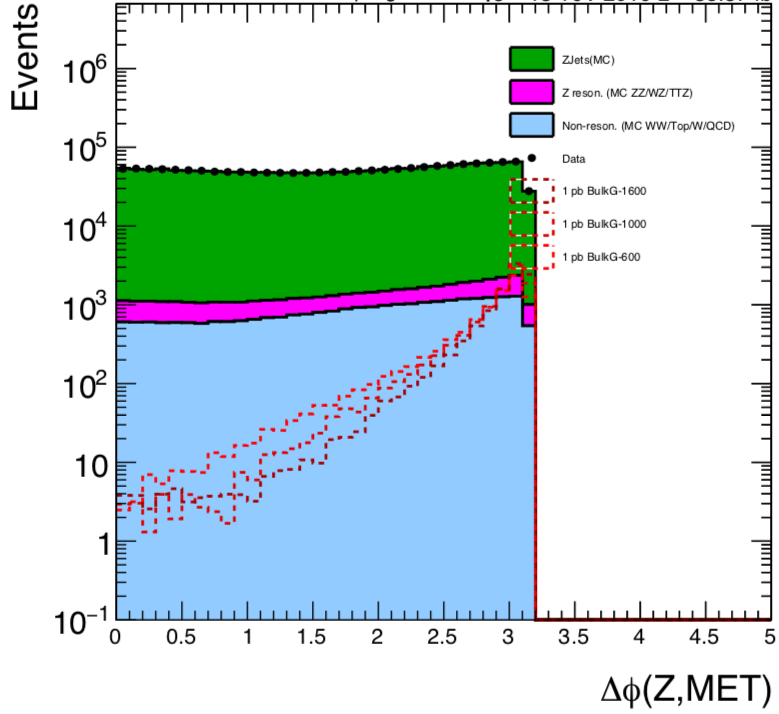
\includegraphics[width=0.75\linewidth]{figures/sel_deltaPhi_ZMET.png}
\caption{$|\Delta \Phi (p_T ^Z ,\ptmiss)|$ distributions for background and signal}
\label{fig:sel_deltphi}
\end{center}
\end{figure}


\vspace{0.3cm}
To summarize, the selection criteria in the signal region are listed below:
\begin{enumerate}
\item Trigger: single muon and single electron triggers as documented in Section~\ref{sec:samples_hlt}
\item Lepton ID and ISO:
  \subitem Muons: Tracker High $p_T$ ID $+$ High $p_T$ ID combination in a muon pair, 
  both muons are also required to pass tracker ISO
  \subitem Electrons: both electrons pass Loose Electron ID and corresponding PF Isolation
\item Lepton acceptance cuts:
  \subitem Muons: Leading  $p_T > 60\GeV$, subleading $p_T > 20\GeV$, both muons in $|\eta| < 2.4$
  \subitem Electrons: Leading $p_T >120\GeV$, subleading $p_T >35\GeV$, both electrons in $|\eta|<2.5$
\item Dilepton pair selection: A pair of same flavor opposite sign
  leptons. The pair with closest invariant mass to the true Z boson mass is selected
\item Z mass window:   $70 < |M_{ll}| < 110\GeV$
\item Z boson: $p_T >100\GeV$
\item Missing $p_T$: $\ptmiss > 50\GeV$
\item $|\Delta \Phi (p_T ^Z ,\ptmiss)|>0.5$
\end{enumerate}

